\chapter{Geometry}

Pixels in the image plane have a direct mapping to the position of the camera in the real world. When we use the approximation of the image we might lose some relevant pices of information such as the depth of the objects in the scene or the speed of objects, which will appear slower the further they are from the camera. 

In this chapter we will introduce the basic concepts of geometry that will allow us to understand the relationship between the camera and the real world.

Typically we represent a point (pixel) as a set of coordinates:

\[ P = [ x, y ]^t = \begin{bmatrix} x \\ y \end{bmatrix}\]

Often convenient to use homogeneous coordinates:
\[ P = [ x, y ]^t = [sx, sy, s]\]

Where \( s \) is a scaling factor, commonly set to 1.0, this will help us when doing transformations.

\[ P = [ x, y ]^t = [x, y, 1]\]

Sometimes we can also omit the " \(^t\) " and write the coordinates as a row vector.

\section{Affine Transformations}

Now formally the pixel is a vector so in general we can apply all the kind of transofmations we want, which usually turn out to be combinations of summations and multiplications. 
The most common transformations are:

\begin{itemize} 
    \item Scaling 
    \item Translation 
    \item Rotation 
    \item Combinations of the above 
\end{itemize}

\subsection{Scaling}

In scaling we take one point or a set of points and we transform them by a multiplaying factor.

\[
\begin{bmatrix}
    x' \\
    y'
    \end{bmatrix}
    =
    \begin{bmatrix}
    c & 0 \\
    0 & c
    \end{bmatrix}
    \begin{bmatrix}
    x \\
    y
    \end{bmatrix}
\]

\begin{figure}[ht]
    \centering
    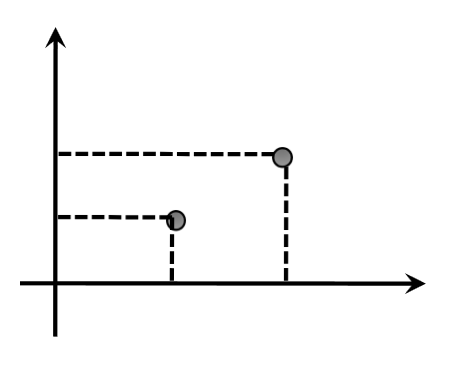
\includegraphics[width=0.3\textwidth]{Figures/scaling.png}
    \caption{Scaling}
    \label{fig:scaling}
\end{figure}

This is a very simple transformation, it can happen that we have not a single coefficient \(c\) but different scaling factors for the different axis.
\[
\begin{bmatrix}
    x' \\
    y'
    \end{bmatrix}
    =
    \begin{bmatrix}
    c_x & 0 \\
    0 & c_y
    \end{bmatrix}
    \begin{bmatrix}
    x \\
    y
    \end{bmatrix}
\]

\subsection{Rotation}

Rotation is the result of applying a rotation angle to the coordinate points, if we go back to the trigonomety we can see that we can use the sine and cosine information of the angle \(\theta\) and we can imagine that if we are rotating a unit vector, the coordinates of the new vector will be the sine and cosine of the angle.

\begin{figure}[ht]
    \centering
    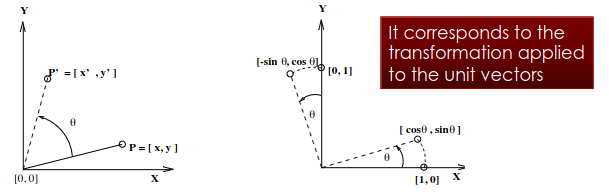
\includegraphics[width=0.75\textwidth]{Figures/rotation.png}
    \caption{Rotation}
    \label{fig:rotation}
\end{figure}

For instance we can see on the horizontal unit vector how the \(x\) gets reduced while a \(y\) component appears correspondin to the sine of the angle.

By the time we have a point that's been shifter by a certain amount \(\theta\), saying that the points rotates equals to keeping the point fixed and rotating the coordinate system by the same amount. The resulting operation that we have in our matrix is the multiplication of the point with the transformation of the unit vectors.

\[
    \begin{bmatrix}
        x' \\
        y'
        \end{bmatrix}
        =
        \begin{bmatrix}
        \cos\theta & -\sin\theta \\
        \sin\theta & \cos\theta
        \end{bmatrix}
        \begin{bmatrix}
        x \\
        y
        \end{bmatrix}
        =
        \begin{bmatrix}
        x \cos\theta - y \sin\theta \\
        x \sin\theta + y \cos\theta
        \end{bmatrix}    
\]

Both scaling and rotation can be constructed using a simple 2 by 2 matrix.
\subsection{Translation}

A translation is simply a shift of the points of our objects into new coordinates.
Just like we can think of rotation as a change in the coordinate system, we can think of translation as a change in the origin of the coordinate system.

If we apply a displacenent vector it's the same as moving the origin of the coordinate system to the new point and we can model this easily:

\( D([x, y]) = [x + x_0, y + y_0] \)

At this point we can't use anymore a 2 by 2 matrix because we have to introduce the two operators \( x_0 \) and \( y_0 \) that are not part of the matrix. 

\[
    \begin{bmatrix}
        x' \\
        y' \\
        \end{bmatrix}
        =
        \begin{bmatrix}
        1 & 0  \\
        0 & 1  \\
        \end{bmatrix}
        \begin{bmatrix}
        x \\
        y \\
        \end{bmatrix}
        +
        \begin{bmatrix}
            x_0 \\
            y_0 \\
        \end{bmatrix}
\]

The new coordinates are nothing but a multiplication of a scaling matrix of facor 1.0 by the coordinates \(x, y\) and then the addition of the translation vector.


To bring the displacement vector inside the matrix we can use the homogeneous coordinates, we can add a third coordinate to the vector and then we can multiply the matrix by the vector.

\[
    \begin{bmatrix}
        x' \\
        y' \\
        1
        \end{bmatrix}
        =
        \begin{bmatrix}
        1 & 0 & x_0 \\
        0 & 1 & y_0 \\
        0 & 0 & 1
        \end{bmatrix}
        \begin{bmatrix}
        x \\
        y \\
        1
        \end{bmatrix}
        =
        \begin{bmatrix}
        x + x_0 \\
        y + y_0 \\
        1
        \end{bmatrix}
\]


\subsection{Rotation, scaling and translation}

Our goal is to be able to map what's happening in the real world to the image plane, we can do this by applying a series of transformations, overall we need to deal with at least 4 parameters:
\begin{itemize} 
    \item One rotation angle (1 parameter)
    \item One scaling factor (1 parameter)
    \item A translation vector (2 parameters)
\end{itemize}

\({}^w P_j = D_{x0,y0} S_s R_\theta {}^i P_i\)

We can describe this combination of transformations with the formula above, where \(D_{x0,y0}\) is the translation matrix, \(S_s\) is the scaling matrix, \(R_\theta\) is the rotation matrix, \(w\) is the world coordinates, \(i\) is the image coordinates and \(j\) a generic point.

\begin{figure}[H]
    \centering
    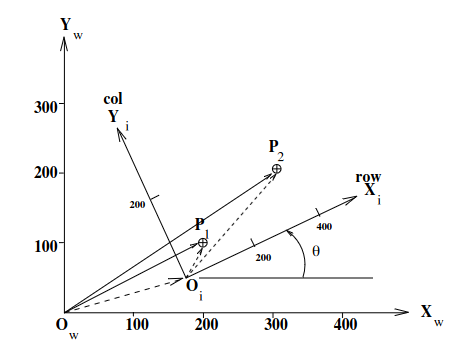
\includegraphics[width=0.75\textwidth]{Figures/comb.png}
    \caption{Here we are applying a translation, a rotation and a scaling to the point \(P\)}
    \label{fig:comb}
\end{figure}

We can write the formula above as a matrix multiplication:

\[
    \begin{bmatrix}
    x_w \\
    y_w \\
    1
    \end{bmatrix}
    =
    \begin{bmatrix}
    1 & 0 & x_0 \\
    0 & 1 & y_0 \\
    0 & 0 & 1
    \end{bmatrix}
    \begin{bmatrix}
        s & 0 & 0 \\
        0 & s & 0 \\
        0 & 0 & 1
    \end{bmatrix}
    \begin{bmatrix}
    \cos\theta & -\sin\theta & 0 \\
    \sin\theta & \cos\theta & 0 \\
    0 & 0 & 1
    \end{bmatrix}
    \begin{bmatrix}
        x \\
        y \\
        1
    \end{bmatrix}
\]

So to obtain the transformation matrix we need to solve a system of euqations with 4 unknowns, the 4 parameters we mentioned before. To obtain 4 equations we can use 2 points called control points ( obtaining \(x_1, y_1\) and \(x_2, y_2\) ), such points must be clearly visible both in the image and in the real world and must be very clear in both planes. Once I have found these two points i'm able to map these coordinates on the image plane.

We keep referring to the transformations in Figure \ref{fig:comb} as \(2D -> 2D \) transformations, this implies I have a ground plane on which i'm working on and a camera plane, the camera plane is the image plane that might be scaled, translated with respect to the ground plane. At the moment we are not considering a rotation of the camera, we are assuming the image plane is parallel to the ground plane.

\begin{figure}[H]
    \centering
    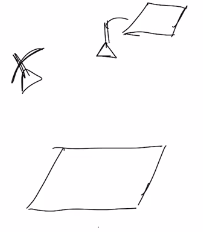
\includegraphics[width=0.2\textwidth]{Figures/planes.png}
    \caption{The camera plane we are considering now is parallel to the ground plane}
    \label{fig:planes}
\end{figure}



\subsection{General Affine Transformations}

Starting from the previous transformations we can see that the 3 matrices are of the same sive and if we compute the product between all of them we can think of these transformations as an end-to-end transformation where we can embed all these parameters in a single matrix.

\[
    \begin{bmatrix}
    u \\
    v \\
    1
    \end{bmatrix}
    =
    \begin{bmatrix}
    a_{11} & a_{12} & a_{13} \\
    a_{21} & a_{22} & a_{23} \\
    0 & 0 & 1
    \end{bmatrix}
    \begin{bmatrix}
        x \\
        y \\
        1
    \end{bmatrix}
\]

This transformation is the set of coefficients, we don't know exactly the contribution of each of the 3 matrices, but it results in a certain trasformation which is represented by what is called in general the \textbf{Camera Matrix}. It tells me exaclty how to move from a certain plane where \(x, y\) lie to where they will be in the camera plane, and vice versa.

We see that we have 6 coefficients instead of the 4 parameters, to determine them it's the same as we did before, with the exception that isntead of 2 we need 3 matching control points which we know the position of in the real world and in the image plane. However finding these points might now be trivial,
the main difficulty is being precise in picking them.

What is usually done is, instead of using the minimum required control points, we pick up more points with the hope that on average we are making a very small mistake, averaging out the errors. This way we might end up with 12, 20 equations and 6 unknowns (an \textit{over-determined system}), our goal is to find the 6 equations that minimize the error. We use the \textit{least-squares method} to find the best solution that minimizes the error.


\[
    \varepsilon (a_{11}, a_{12}, a_{13}, a_{21}, a_{22}, a_{23}) = 
\sum_{j=1}^{n} (a_{11}x_j + a_{12}y_j + a_{13} - u_j)^2 
+ (a_{21}x_j + a_{22}y_j + a_{23} - v_j)^2
\]


What we are trying to get is to find the best configuration of these coefficients in a way that the difference between what's expected from the transformation and what's observed is minimized. The resulting equation system is:

\[
    \begin{bmatrix}
        \sum x^2_j & \sum x_jy_j & \sum x_j & 0 & 0 & 0 \\
        \sum x_jy_j & \sum y^2_j & \sum y_j & 0 & 0 & 0 \\
        0 & 0 & 0 & \sum x^2_j & \sum x_jy_j & \sum x_j \\
        0 & 0 & 0 & \sum x_jy_j & \sum y^2_j & \sum y_j \\
        0 & 0 & 0 & \sum x_j & \sum y_j & \sum 1 
    \end{bmatrix}
    \begin{bmatrix}
        a_{11} \\
        a_{12} \\
        a_{13} \\
        a_{21} \\
        a_{22} \\
        a_{23}
    \end{bmatrix}
    =
    \begin{bmatrix}
        \sum x_ju_j \\
        \sum y_ju_j \\
        \sum u_j \\
        \sum x_jv_j \\
        \sum y_jv_j \\
        \sum v_j
    \end{bmatrix}
\]

The solution is found by computing the minimum of the error, or in other terms compute the \textit{partial derivative} with respect to each unknown and set them to zero, making sure the error between the result of the transformation and the observed points is minimized.

And this is how the whole thing works, how we determine the \textbf{2D camera matrix} used to map the real world plane to the camera plane. Remembder that the reference are two different planes one on top of the other, we don't have full 3D rotations \textit{yet}.

\section{Going 3D}

We are now moving to more general solutions, we can't expect from the system we'll take in consideraton to end up in the easy scenario where the two planes are parallel and facing each other.
More in general what happens is that the image plane we are dealing with it's something that results from a generic camera prospective where what we see in the image plane is something that look more like shown in Figure \ref{fig:3d}.

\begin{figure}[h!]
    \centering
    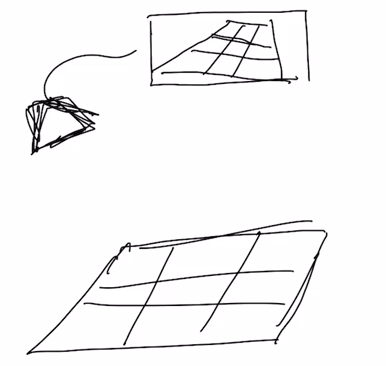
\includegraphics[width=0.2\textwidth]{Figures/3d.png}
    \caption{A generinc 3D scenario.}
    \label{fig:3d}
\end{figure}

We need to go thru a process called \textbf{calibration} where we'll need to determined the so called \textbf{intrinsic} and \textbf{extrinsic} parameters of the camera. The projections that we have seen so far won't be enough to describe the 3D world, we'll need to add an \textit{additional view} to make possible to determiine the unique 3D coordinates \(X Y Z\) that are necessary to describe the position of a point in the real world. With that additional information I can do many tasks:

\begin{itemize} 
    \item Point Clouds
    \item Structure From Motion
    \item Mesh Reconstruction
\end{itemize}

\subsection{Intrinsic and Extrinsic Parameters}

\begin{itemize} 
    \item\textit{Intrisic parameters} refer to the specific characteristics of the camera, such as the focal length, the distortion of the lens, the position of the principal point, etc. These parameters are fixed and don't change with the position of the camera. They are necessary because we want to link the pixel coordinates with the corresponding coordinates in the camera coordinates system.

    \item\textit{Extrinsic parameters} refer to the position of the camera in the real world, such as the rotation and translation of the camera with respect to the world coordinates. These parameters are not fixed and change with the position of the camera.
\end{itemize}

When we try to estimate these parameters we go thru a process called \textbf{calibration}, where we try to find a suitable matrix which helps us mapping the points in the real world to what we see thru the camera.

\subsection{3D Affine Transformations}

At this point we need to go through a the transformations that we have seen in the 2D case, extending them by adding a new dimension. The main difference is that our starting point is a set of 3D coordinates.

\[ [P_x, P_y, P_z] \rightarrow  [sP_x, sP_y, sP_z, s] \]

Also in this case we move from a 3D vector to a 4D vector with the addition of the scaling factor of the homomogeneous coordinates.

Now we have a system for each camera so a triplet of coordinates for Camera 1 and a triplet of coordinates for Camera 2, these two cameras are looking at the world coordinates, in some cases it could be interesing to also know the coordinates of the model in the world (although it's not common). We end up with

\begin{itemize} 
    \item Model coordinates
    \item World coordinates
    \item Camera 1 coordinates
    \item Camera 2 coordinates
\end{itemize}

\begin{figure}[H]
    \centering
    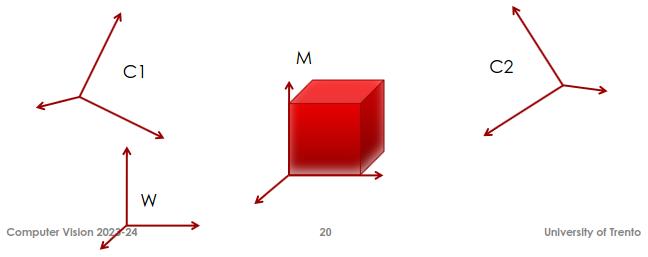
\includegraphics[width=0.8\textwidth]{Figures/coo.png}
    \caption{The new model with two camera views.}
    \label{fig:coo}
\end{figure}

We can see all these 4 systems linked by a transformation, which is nothing more than a rotation-translation to go from any of the 3 systems to the other. At the end it means that we need to deal with a rotation matrix and a translation vector.


\({}^wP = T R {}^mP\) and same for \({}^1P\) and \({}^2P\).

Where T is a translation vector and R a rotation matrix. It must be noted that the point seen from the first camera and the second camera might be different from the second camera, both in terms of coordinates and in the sense that Camera 1 and Camera 2 might have opposite views, meaning that there might be no one-to-one mapping of all points, there's a supset of points that's visible from both cameras, we'll be able to recontruct the 3D position only for the points visible from both cameras.


NB:
The notation for the next section will be \({}^kP_j\) where \(k\) is the camera number and \(j\) is the point number.


\subsection{3D Translation}

Across the two views in order to move the point from a camera to the other we apply a translation,
it consists of applying a translation \(x_0, y_0, z_0\) to the point and no scaling.

\[
  {}^2P = T(x_0, y_0, z_0) {}^1P 
\]

\[
    \begin{bmatrix}
        {}^2P_x \\
        {}^2P_y \\
        {}^2P_z \\
        1
    \end{bmatrix}
    =
    \begin{bmatrix}
        1 & 0 & 0 & x_0 \\
        0 & 1 & 0 & y_0 \\
        0 & 0 & 1 & z_0 \\
        0 & 0 & 0 & 1
    \end{bmatrix}
    \begin{bmatrix}
        {}^1P_x \\
        {}^1P_y \\
        {}^1P_z \\
        1
    \end{bmatrix}   
\]

\subsection{3D Scaling}

Here, similarly to the previous case, we can have different scaling factors although usually we have the same scaling factor for all the axis.

\[
  {}^2P = S(s_x, s_y, s_z) {}^1P 
\]

\[
    \begin{bmatrix}
        {}^2P_x \\
        {}^2P_y \\
        {}^2P_z \\
        1
    \end{bmatrix}
    =
    \begin{bmatrix}
        s_x & 0 & 0 & 0 \\
        0 & s_y & 0 & 0 \\
        0 & 0 & s_z & 0 \\
        0 & 0 & 0 & 1
    \end{bmatrix}
    \begin{bmatrix}
        {}^1P_x \\
        {}^1P_y \\
        {}^1P_z \\
        1
    \end{bmatrix}   
\]

\subsection{3D Rotation}

In terms of rotation, things become a little more complicated, we don't have a single rotation (in the 2D space we have to deal with a single angle) but since now we have an additional axis we have a rotation arounf the three axis, if we want to do the same analysis as we did in the 2D case with the unit vector we end up with three matrices of coefficients that describe the rotation around each of the three axis.

\begin{multicols}{2}

    

\[
  {}^2P = R(X, \varTheta ) {}^1P 
\]

\[
    \begin{bmatrix}
        {}^2P_x \\
        {}^2P_y \\
        {}^2P_z \\
        1
    \end{bmatrix}
    =
    \begin{bmatrix}
        1 & 0 & 0 & 0 \\
        0 & \cos\theta & -\sin\theta & 0 \\
        0 & \sin\theta & \cos\theta & 0 \\
        0 & 0 & 0 & 1
    \end{bmatrix}
    \begin{bmatrix}
        {}^1P_x \\
        {}^1P_y \\
        {}^1P_z \\
        1
    \end{bmatrix}   
\]

\[
  {}^2P = R(Y, \varTheta ) {}^1P 
\]

\[
    \begin{bmatrix}
        {}^2P_x \\
        {}^2P_y \\
        {}^2P_z \\
        1
    \end{bmatrix}
    =
    \begin{bmatrix}
        \cos\theta & 0 & \sin\theta & 0 \\
        0 & 1 & 0 & 0 \\
        -\sin\theta & 0 & \cos\theta & 0 \\
        0 & 0 & 0 & 1
    \end{bmatrix}
    \begin{bmatrix}
        {}^1P_x \\
        {}^1P_y \\
        {}^1P_z \\
        1
    \end{bmatrix}   
\]
\end{multicols}
\[
  {}^2P = R(Z, \varTheta ) {}^1P 
\]

\[
    \begin{bmatrix}
        {}^2P_x \\
        {}^2P_y \\
        {}^2P_z \\
        1
    \end{bmatrix}
    =
    \begin{bmatrix}
        \cos\theta & \sin\theta & 0 & 0 \\
        -\sin\theta & \cos\theta & 0 & 0 \\
        0 & 0 & 1 & 0 \\
        0 & 0 & 0 & 1
    \end{bmatrix}
    \begin{bmatrix}
        {}^1P_x \\
        {}^1P_y \\
        {}^1P_z \\
        1
    \end{bmatrix}   
\]

\subsection{3D General Configuration}

Our goal is to then put everything together in a single matrix, this is the generic 3D affine transformation that maps a point in the 3D coordinates of the first system to the 3D coordinates of the second system.

\[
    \begin{bmatrix}
        {}^2P_x \\
        {}^2P_y \\
        {}^2P_z \\
        1
    \end{bmatrix}
    =
    \begin{bmatrix}
       r_{11} & r_{12} & r_{13} & t_x \\
       r_{21} & r_{22} & r_{23} & t_y \\
       r_{31} & r_{32} & r_{33} & t_z \\
        0 & 0 & 0 & 1
    \end{bmatrix}
    \begin{bmatrix}
        {}^1P_x \\
        {}^1P_y \\
        {}^1P_z \\
        1
    \end{bmatrix}   
\]

It's some sort of a camera matrix, but at this point we are dealing with something that return 3D coordinates and unfurtunately doesn't help us much because at the end what we have is an image plane where the coordinates are only rows and columns, \(x, y\). It means that we need to further modify this matrix in order to end up with a representation that 2D. We need to add to our transformation what are the proprieties of the camera, that give us the opportunity to move from the 3D coordinates (in our case the world \(W\)) to a 2D plane \(I\).

\[
    {}^IP = {}^I_W C^WP
\]

This matrix here flattens the information and returns a 2D vector corresponding to the position in the rows and columns of the image plane and this happens by adopting a 3 by 4 matrix that gives us the chance to move from the 3D world to the 2D camera coordinates.

\[
    \begin{bmatrix}
        s^IP_r \\
        s^IP_c \\
        s
    \end{bmatrix}
    =
    {}^I_W C^W
    \begin{bmatrix}
        {}^WP_x \\
        {}^WP_y \\
        {}^WP_z \\
        1
    \end{bmatrix}  
    = 
    \begin{bmatrix}
        c_{11} & c_{12} & c_{13} & c_{14} \\
        c_{21} & c_{22} & c_{23} & c_{24} \\
        c_{31} & c_{32} & c_{33} & 1
    \end{bmatrix}
    \begin{bmatrix}
        {}^WP_x \\
        {}^WP_y \\
        {}^WP_z \\
        1
    \end{bmatrix}
\]

unfurtunately we are still not happy because while it's true that we have the camera coordinates on the image plane but that would be a continuous hypotetical image plane where we do not have pixels (basically an implementation of the pinhole, but it's not discretized). It's a 2D representation but it's not the one that we want.

We need to work again on these transformation moving from the camera to some additional coordinates:
\textit{(While important the following part till the end of the section is was covered briefly)}
\[
    \begin{bmatrix}
        {}^CP_x \\
        {}^CP_y \\
        {}^CP_z \\
        1
    \end{bmatrix}
    =
    \begin{bmatrix}
       r_{11} & r_{12} & r_{13} & t_x \\
       r_{21} & r_{22} & r_{23} & t_y \\
       r_{31} & r_{32} & r_{33} & t_z \\
        0 & 0 & 0 & 1
    \end{bmatrix}
    \begin{bmatrix}
        {}^WP_x \\
        {}^WP_y \\
        {}^WP_z \\
        1
    \end{bmatrix}   
\]

\[
    {}^CP = {}^C_W TR(\alpha, \beta, \gamma, t_x, t_y, t_z) {}^WP
\]

\({}^CP\) is about the \textit{camera coordinates}, and
not the \textit{image coordinates} \({}^FP\), we need to project these on the image coordinates and successively discretize them in the pixel coordinates.

\[
    {}^FP = {}^F_C \varPi (f) {}^CP
\]

\[
    {}^FP = {}^F_C \varPi (f) TR(\alpha, \beta, \gamma, t_x, t_y, t_z) {}^WP
\]


\[
    \begin{bmatrix}
        s^FP_r \\
        s^FP_c \\
        s
    \end{bmatrix}
    =
    \begin{bmatrix}
        d_{11} & d_{12} & d_{13} & d_{14} \\
        d_{21} & d_{22} & d_{23} & d_{24} \\
        d_{31} & d_{32} & d_{33} & 1
    \end{bmatrix}
    \begin{bmatrix}
        {}^WP_x \\
        {}^WP_y \\
        {}^WP_z \\
        1
    \end{bmatrix}
\]

The conversion from mm to pixel consists of a scaling factor related to the real size of the pixels where \(d_x\) is the size of the pixel in the x direction and \(d_y\) is the size of the pixel in the y direction.

\[
  {}^IP={}^I_F S^F P  
\]


\[
    {}^I_F S^F
    = 
    \begin{bmatrix}
        0 & -1/d_y & 0\\
        1/d_x & 0 & 0\\
        0 & 0 & 1
    \end{bmatrix}
\]

The minus sign is due to the fact that the origin is usually bottom left but in the image it's top left so we flip the coordinates.

Overall in order to get the position rows and columns on the image plane we need to go from 3D generic world coordinates to the camera coordinates than we need the intrinsic information of the camera and then we need to discretize the pixels.

\[
  [p_r, p_c]^T = {}^IP = {}^I_F S^F_C \varPi (f)^C_W TR(\alpha, \beta, \gamma, t_x, t_y, t_z) {}^WP
\]

And we finally get out final camera matrix:

\[
    \begin{bmatrix}
        s^Ip_r \\
        s^Ip_c \\
        s
    \end{bmatrix}
    = 
    \begin{bmatrix}
        c_{11} & c_{12} & c_{13} & c_{14} \\
        c_{21} & c_{22} & c_{23} & c_{24} \\
        c_{31} & c_{32} & c_{33} & 1
    \end{bmatrix}
    \begin{bmatrix}
        {}^WP_x \\
        {}^WP_y \\
        {}^WP_z \\
        1
    \end{bmatrix}
\]

At the end the entire iter of transformations that we use to go from the 3D points in space to the pixel coordinates is included in the 3 x 4 camera matrix. It means that overall we need to compute 11 parameters (we are not considering the scaling parameter) and in order to create a reasonable mapping of the points we need to compute these coefficients. We'll see that the process that we follow to obtain the coefficients if basically the same as the 2D case.

\section{Calibration}

What we did till now was introducing some geometry problems by saying that what we want to do is to find the relationships between different domains: what happens in the real world and what happens on the camera side. During the process of acquisition the relationships between the two domains change through rotations, translations and scaling. To describe them we came up with a \textit{camera matrix} that helps us mapping what happens in the real world with what happens in the camera.

The \(3 \times 4\) camera matrix contains 12 coefficients, 11 of which are unknown, we need to find them in order to map the points in the real world to the image plane. The process of finding these coefficients is called \textbf{calibration}.

In order to determine the 11 unknowns we need 6 matching pairs (12 equations) which are enough to solve the system. To pick them we do the same as in the simpler 2D case, we choose points in the real world for whom we know the coordinates and we choose the same points in the image plane, we need to be very precise in picking these points so usually we pick an \textit{higher number} of points to average out the errors.

It's common to use an object of known geometry (a calibration patter) for which we know the relative position of the points and for this we compute the matching.


\subsection{Calibration Procedure}

As we have seen before, we have the points in the 3D world, we have the matching 2D projections and we can start constructing our equations system.


Given a 3D point \([{}^WP_x {}^WP_y {}^WP_z]\) and its projection \([{}^IP_r {}^IP_c] = [u v]\) for each point in the calibration process we can write the system of equations:
\setcounter{MaxMatrixCols}{20}

\[
    \begin{bmatrix}
        x_j & y_j & z_j & 1 & 0 & 0 & 0 & 0 & -x_ju_j & -y_ju_j & -z_ju_j \\
        0 & 0 & 0 & 0 & x_j & y_j & z_j & 1 & -x_jv_j & -y_jv_j & -z_jv_j \\
    \end{bmatrix}
    \begin{bmatrix}
        c_{11} \\
        c_{12} \\
        c_{13} \\
        c_{14} \\
        c_{21} \\
        c_{22} \\
        c_{23} \\
        c_{24} \\
        c_{31} \\
        c_{32} \\
        c_{33} \\
    \end{bmatrix}
    =
    \begin{bmatrix}
        u_j \\
        v_j
    \end{bmatrix}
\]

As usual our goal is to rely on the least square to find the configuration of the matrix the minimizes the error between the observed points and the points that we expect from the transformation, the error between the actual image point measurements and the world points comes from

\[
    {}^IP={}^I_WC^WP  
\]


\begin{figure}[H]
    \centering
    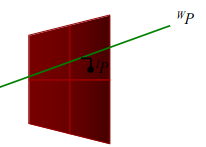
\includegraphics[width=0.4\textwidth]{Figures/proj.png}
    \caption{Error in the projection.}
    \label{fig:proj}
\end{figure}

In an ideal world all the points coming from the real world all the points are being projected on the center of projection, we can trace  the ray through the camera plane and that's it. In the real world we make mistakes, and as shown in Figure \ref{fig:proj} the points are not exactly where we expect them to be, the error is the difference between the expected and the observed points, what we are triyng to do is to minimize this error.

\subsection{Computing the 3D position of a point}

Now we are in the situation where we can map points in the real world on the image plane and can get closer to one of our biggest issues: with just a single camera we cannot compute the full 3D coordinates of a point. If we add an additional camera we can have two different systems, at that point we have 4 equations (2 for each camera) and if we know the camera matrixes for each camera we can come up with the 3D position of the point.

Given a generic point \([x, y, z] \) and given two projections \([r_1, c_1]\) and \([r_2, c_2]\) we can write:

\begin{multicols}{2}

    \[
        \begin{bmatrix}
            sr_1 \\
            sc_1 \\
            s
        \end{bmatrix}  
        =
        \begin{bmatrix}
            b_{11} & b_{12} & b_{13} & b_{14} \\
            b_{21} & b_{22} & b_{23} & b_{24} \\
            b_{31} & b_{32} & b_{33} & 1
        \end{bmatrix}
        \begin{bmatrix}
            x \\
            y \\
            z \\
            1
        \end{bmatrix}
    \]

    \[
        \begin{bmatrix}
            tr_2 \\
            tc_2 \\
            t
        \end{bmatrix}  
        =
        \begin{bmatrix}
            c_{11} & c_{12} & c_{13} & c_{14} \\
            c_{21} & c_{22} & c_{23} & c_{24} \\
            c_{31} & c_{32} & c_{33} & 1
        \end{bmatrix}
        \begin{bmatrix}
            x \\
            y \\
            z \\
            1
        \end{bmatrix}
    \]
\end{multicols}

To compute and recontruct the 3D posintion of the point we can solve the system of equations and find a solution.

If we assume we have the projections we know that they are subject to a certain error and that error caused by an approximation of the projection can be seen in the real world as an error in the intersection of the two rays.


\begin{figure}[H]
    \centering
    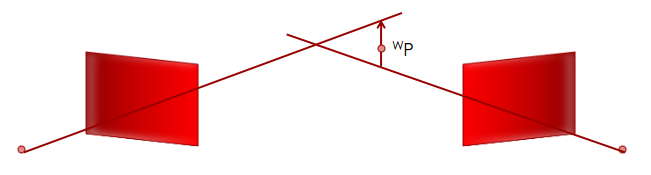
\includegraphics[width=0.7\textwidth]{Figures/inter.png}
    \caption{Error in the intersection.}
    \label{fig:inter}
\end{figure}

Usually what's done is to take the distance between the two lines and use the middle point as the 3D position of the point. 

\section{The Binocular Stereo}

As the name suggests it's basically a system that looks like Figure \ref{fig:inter} where we have two cameras and we try to come up with few equations to model that situation, which by no coincidence is the same system humans are equipped with. It can be scaled up with multiple cameras but the idea is the same as it becomes a pairwise binocular system. The computation of the 3D position of a points usually goes through 2 steps:

\begin{itemize}
    \item Computation of the correspondencies (main source of error)
    \item Reconstruction of the 3D position (basically deterministic)
\end{itemize}

The conditions for a binocular system is that overall we have two cameras positioned anywhere in the real world pointing at a scene where there's an area that overlaps. From the area that's visible by both camera I can compute the reconstruction.

\begin{figure}[H]
    \centering
    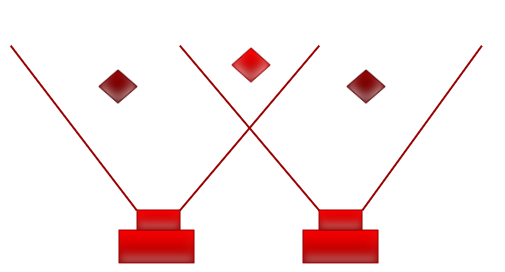
\includegraphics[width=0.6\textwidth]{Figures/binoc.png}
    \caption{This is also a specific case where both cameras are parallel and aligned (coplanar) as in most commercial stereo systems.}
    \label{fig:binoc}
\end{figure}




\begin{figure}[h!]
    \centering
    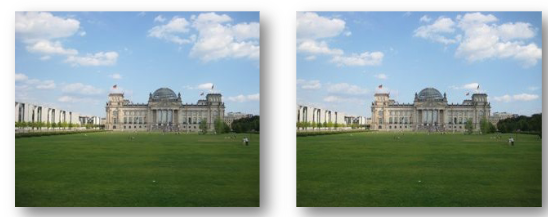
\includegraphics[width=0.6\textwidth]{Figures/coplan.png}
    \caption{Coplanar views.}
    \label{fig:coplan}
\end{figure}

In the case of coplanar cameras the difference between the views will be just a small offset as shown in Figure \ref{fig:coplan}. Points will result shifted, and the shift will depend on the depth of the point, the further the point the smaller the shift, this leads to the \textbf{parallax}, apparent motion.  

\subsection{Computing Correspondencies}

The first step is to compute the correspondencies, in order to do so we need to find those points that are representing the same portion of the real world and this is possible mostly because if we have a good acquisition system the distance is not too big, it's normal to look for a certain match in the local area around the point of interest.

We can rely also on the \textbf{Epipolar Constraint} which tells us that the correspondencies can be met along a horizontal line called the \textit{epipolar line}.

\subsection{Stereo Vision and Epipolar Geometry}

\begin{figure}[H]
    \centering
    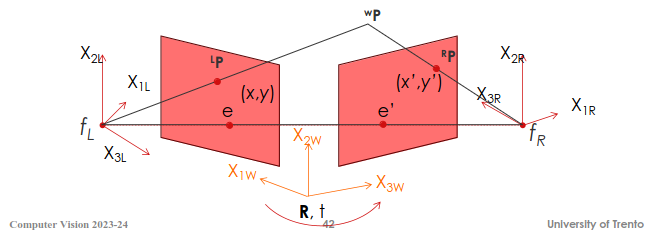
\includegraphics[width=0.75\textwidth]{Figures/stereo.png}
    \caption{A generic stereo system.}
    \label{fig:stereo}
\end{figure}

This is a slightly more complex system compared to the coplanar one. We have a Left and a Right camera, both will have their camera coordinates system and we also have to coordinates of the real world. Our objective is to start from a point aviable in the real world , look where the point is being projected in the first and second camera and use the information of this projection to infer the coordinates of \({}^WP\).

\[
    \begin{bmatrix}
        x \\
        y
    \end{bmatrix}
    \begin{bmatrix}
        x' \\
        y'
    \end{bmatrix}
    \rightarrow 
    \begin{bmatrix}
        X \\
        Y \\
        Z
    \end{bmatrix}
\]

We need to go through the \textbf{Epipolar Geometry}.

\begin{figure}[H]
    \centering
    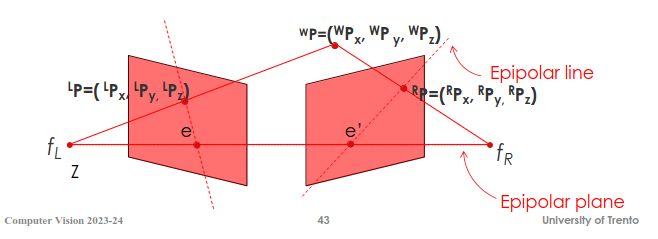
\includegraphics[width=0.75\textwidth]{Figures/epipolar.png}
    \caption{Epipolar geometry.}
    \label{fig:epipolar}
\end{figure}

The \textbf{epipolar plane} is what connects the  \({}^WP\) with the two cameras, this plane can be seen as something anchored to axis \(f_L\) and \(f_R\), since they dont move, depending of where the point is in the world what chances in the inclination of the plane. The intersection in between the epipolar plane and the image plane is what we call the \textbf{epipolar lines}. The points \(e\) and \(e'\) are the \textbf{epipoles} and they are the intersection of the epipolar lines with the image plane, they are useful because, for example, as the \({}^WP\) moves along it's projection line on \(f_R\) (basically the ray that goes from \(f_R\) to \({}^WP\)) it's projection on the right image plane will remain the same meanwhile its projection on the left image plane will move exlusively along the epiploar line, so we \textit{know} that we only need to look in that area to find the correspondence. 

\begin{figure}[H]
    \centering
    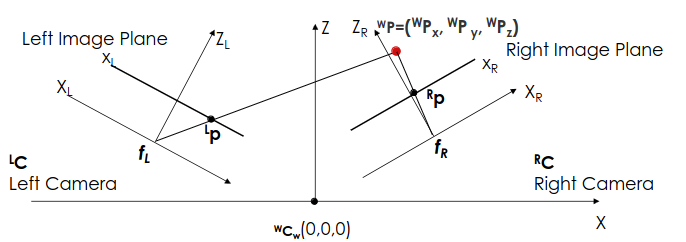
\includegraphics[width=0.75\textwidth]{Figures/epipolar_above.png}
    \caption{The same system from above.}
    \label{fig:epipolar_above}
\end{figure}

We have 


\[{}^RP = ({}^RP_x, {}^RP_y, {}^RP_z) \;\;\;\;
{}^LP = ({}^LP_x, {}^LP_y, {}^LP_z)\;\;\;\;
{}^WP = ({}^WP_x, {}^WP_y, {}^WP_z)\]


\[
    {}^RP = {}^RR{}^WP+{}^RT
\]
\[
    {}^LP = {}^LR{}^WP+{}^LT  
\]

We know that the point seen from the camera systems will be the result of a some roto-translations of the point in the real world to the coordinate system of the cameras, \(R\) and \(T\) are related to the extrinsic parameters of the cameras.

The only common term between the two last equations is \({}^WP\) so we can sobstitute and get:

\[
    {}^LP = {}^LR{}^RR^{-1}{}^RP-{}^LR{}^RR^{-1}{}^RT+{}^LT
\]

\[
    = M^RP+B
\]

Where the term \(M\) that multiplies the \({}^RP\) and a term \(B\). This tells us that in between the \(L\) and the \(R\) we have a roto-translation. Using the simplified perspective projections (Z > f) we obtain the coordinates on the two image planes:

\begin{multicols}{2}

\(
    {}^Lp_x = f\frac{{}^LP_x}{{}^LP_z}  
\) \\
\(
    {}^Lp_y = f\frac{{}^LP_y}{{}^LP_z}
\)

\end{multicols}

\begin{multicols}{2}

\(
    {}^Rp_x = f\frac{{}^RP_x}{{}^RP_z}  
\) \\
\(
    {}^Rp_y = f\frac{{}^RP_y}{{}^RP_z}
\)
    
\end{multicols}

from which we obtain 

\[
    \frac{{}^LP_z}{f}
    \begin{bmatrix}
        {}^Lp_x \\
        {}^Lp_y \\
        f
    \end{bmatrix}
    =
    \frac{{}^RP_z}{f}
    M
    \begin{bmatrix}
        {}^Rp_x \\
        {}^Rp_y \\
        f 
    \end{bmatrix}
    + B
\]
